\section{Observer Class Reference}
\label{classObserver}\index{Observer@{Observer}}
Inheritance diagram for Observer:\begin{figure}[H]
\begin{center}
\leavevmode
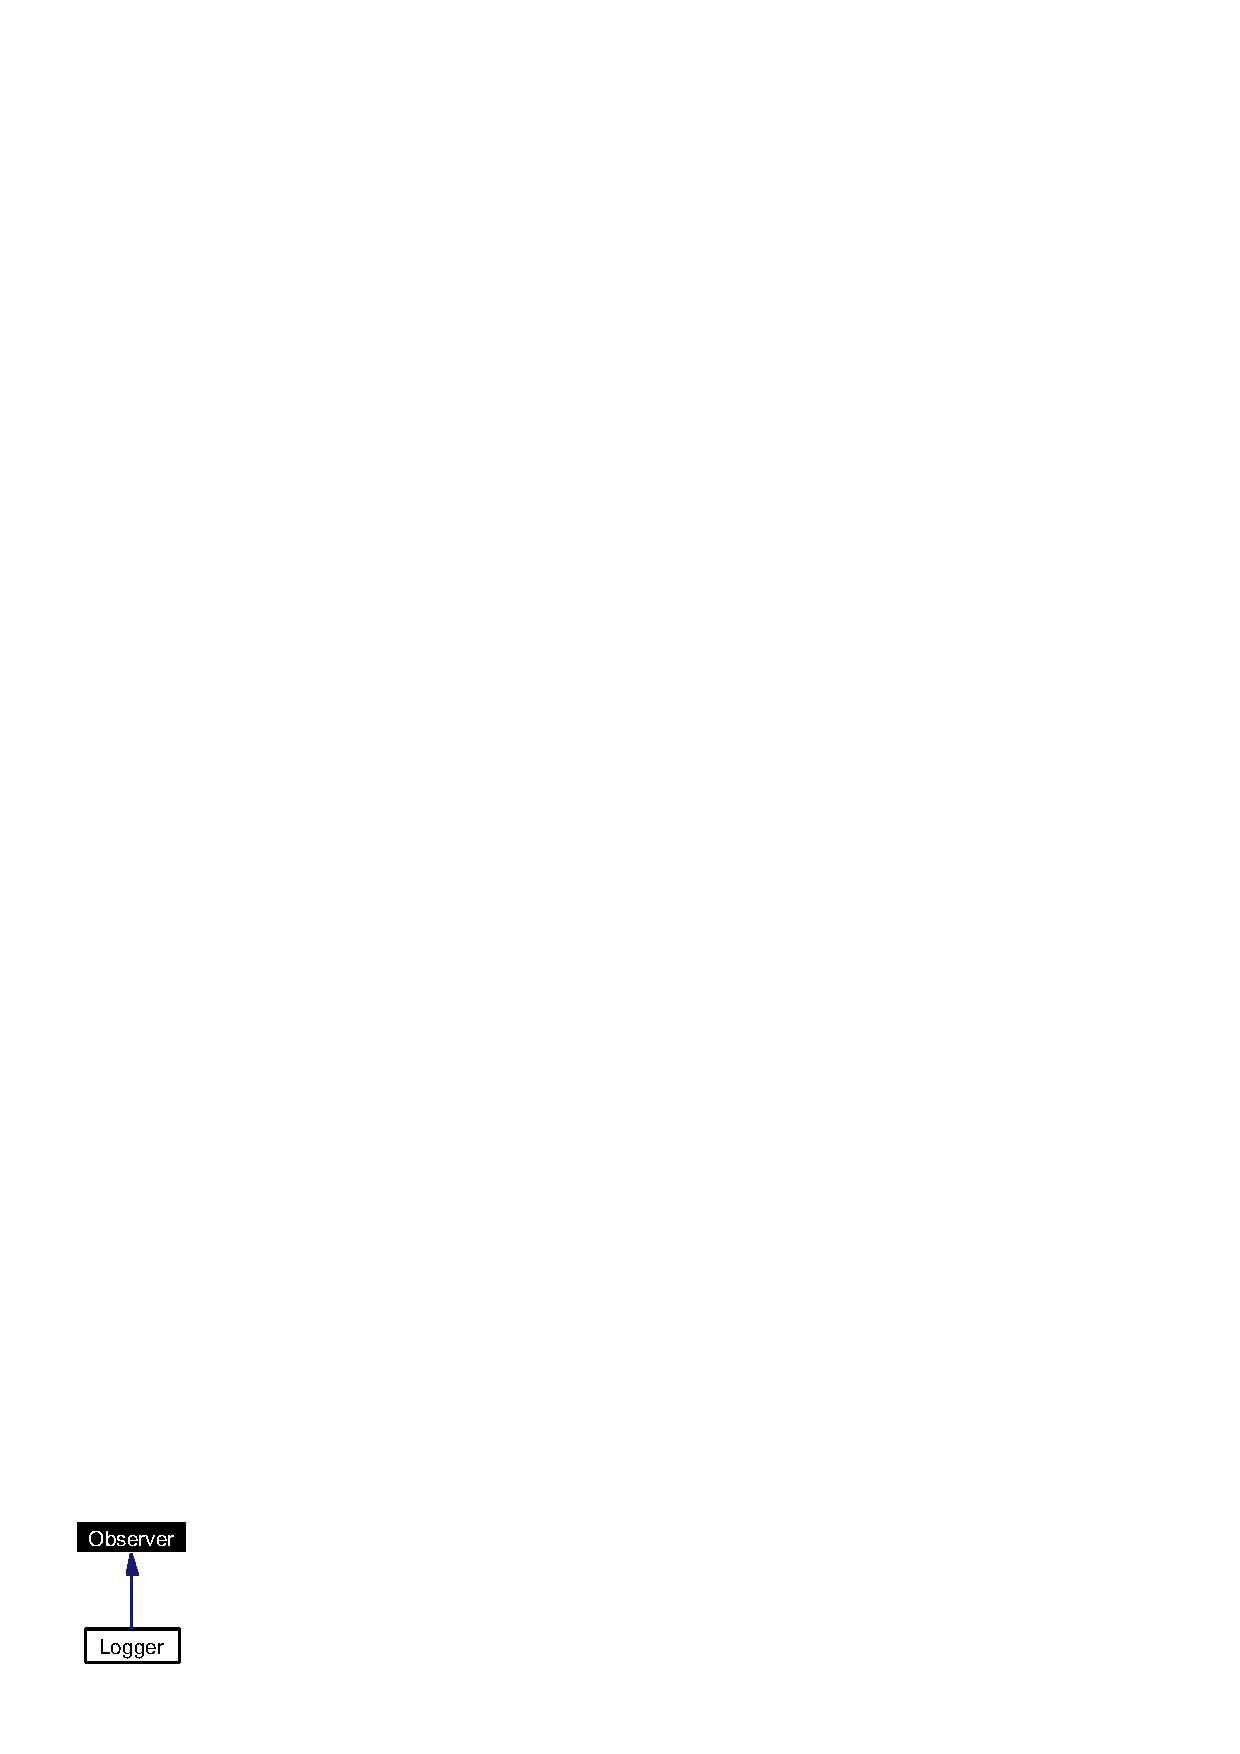
\includegraphics[width=45pt]{classObserver__inherit__graph}
\end{center}
\end{figure}
\subsection*{Public Member Functions}
\begin{CompactItemize}
\item 
{\bf notify} (\$event, \$msg)\label{classObserver_a0}

\end{CompactItemize}
\subsection*{Public Attributes}
\begin{CompactItemize}
\item 
{\bf \$\_\-observer\-Id} = ''\label{classObserver_o0}

\begin{CompactList}\small\item\em This will be assigned by an observable object when attaching. \item\end{CompactList}\end{CompactItemize}


\subsection{Detailed Description}
Methods to override: notify(\$event, \$msg) This implements the Observer design pattern defining the Observer class. Observer objects can be \char`\"{}attached\char`\"{} to {\bf Observable}{\rm (p.\,\pageref{classObservable})} objects to listen for a specific event. Example:

\$log = new {\bf Logger}{\rm (p.\,\pageref{classLogger})}(\$logfile); //Logger extends Observer \$foo = new Foo(); //Foo extends {\bf Observable}{\rm (p.\,\pageref{classObservable})} \$foo-$>$attach('moo',\$log); //Now \$log observers 'moo' events in \$foo class of \$foo-$>$attach\_\-all(\$log); // Same but all events are listened 



Definition at line 19 of file Observer.php.

The documentation for this class was generated from the following file:\begin{CompactItemize}
\item 
Observer.php\end{CompactItemize}
